\subsection{Flaming auroral arcs}\label{sec:fusflame}
Flaming aurora manifests as rapidly increasing peak brightness altitude.
The effect can have an appearance like the rapidly rising flames of a campfire, leading to the name for this auroral morphology.
The driving factor behind flaming aurora is dispersive Alfvén waves.
The high energy precipitating particles arrive first in the auroral altitudes of the ionosphere, followed $\sim \unit[100]{ms}$ later by the lower energy particles. 

An example flaming auroral arc occurred at PFISR on March 1, 2011 near 10:06 UTC. 
Figure~\ref{fig:20110301a}(a) shows pre-Alfvénic arc configuration. 
F-region irregularities starting below \unit[300]{km} and rising up to \unit[600]{km} within two seconds are observed in Figure~\ref{fig:20110301a}(b) ISR power with the arrival of high-energy dispersive Alfvénic particles. 
\unit[400]{ms} later in Figure~\ref{fig:20110301a}(c), the low-energy Alfvénic flux dominates as the apparent peak altitude of prompt emissions rises rapidly. 
Figure~\ref{fig:20110301b}(a) shows the ion-line during the NEIAL altitude climb, with (g) after the NEIAL rose to a more steady altitude.
A few seconds later in Figure~\ref{fig:20110301a}(d), the Alfvénic particle packet has vanished.
Figure~\ref{fig:20110301b}(c) shows the ion-line spectrum without NEIALs present.
Observe that two more NEIAL events occurred before and after the video, but due to the human-initiated record cycle, they were not recorded with video.
\begin{sidewaysfigure}\centering
    % Video
    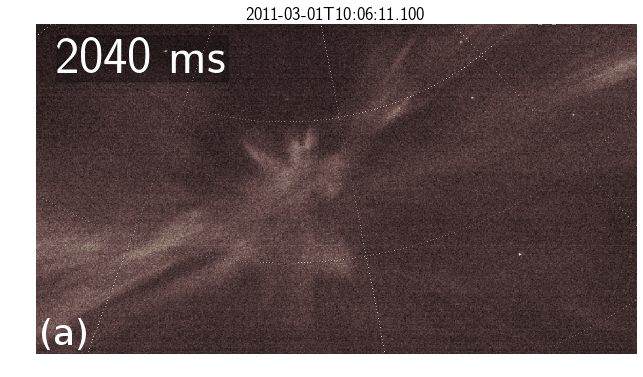
\includegraphics[width=0.19\columnwidth,trim=30 0 200 0,clip]{gfx/2011-03-01/2040}
    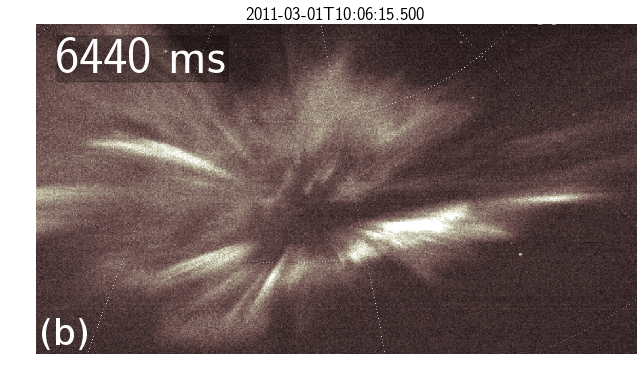
\includegraphics[width=0.261\columnwidth,trim=30 0 60 0,clip]{gfx/2011-03-01/6440}
    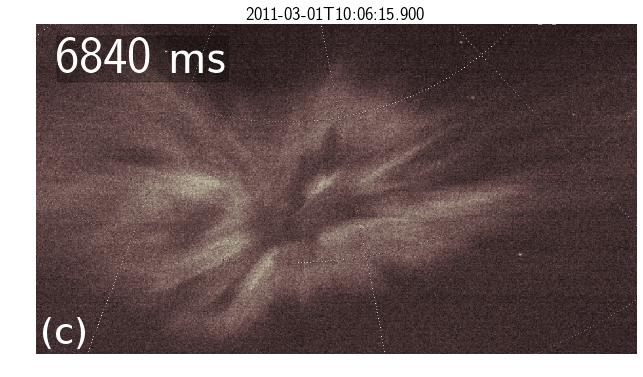
\includegraphics[width=0.261\columnwidth,trim=30 0 60 0,clip]{gfx/2011-03-01/6840}        
    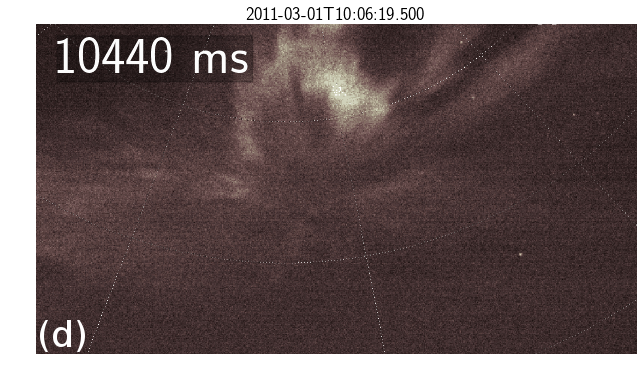
\includegraphics[width=0.261\columnwidth,trim=30 0 60 0,clip]{gfx/2011-03-01/10440}
    % Power
    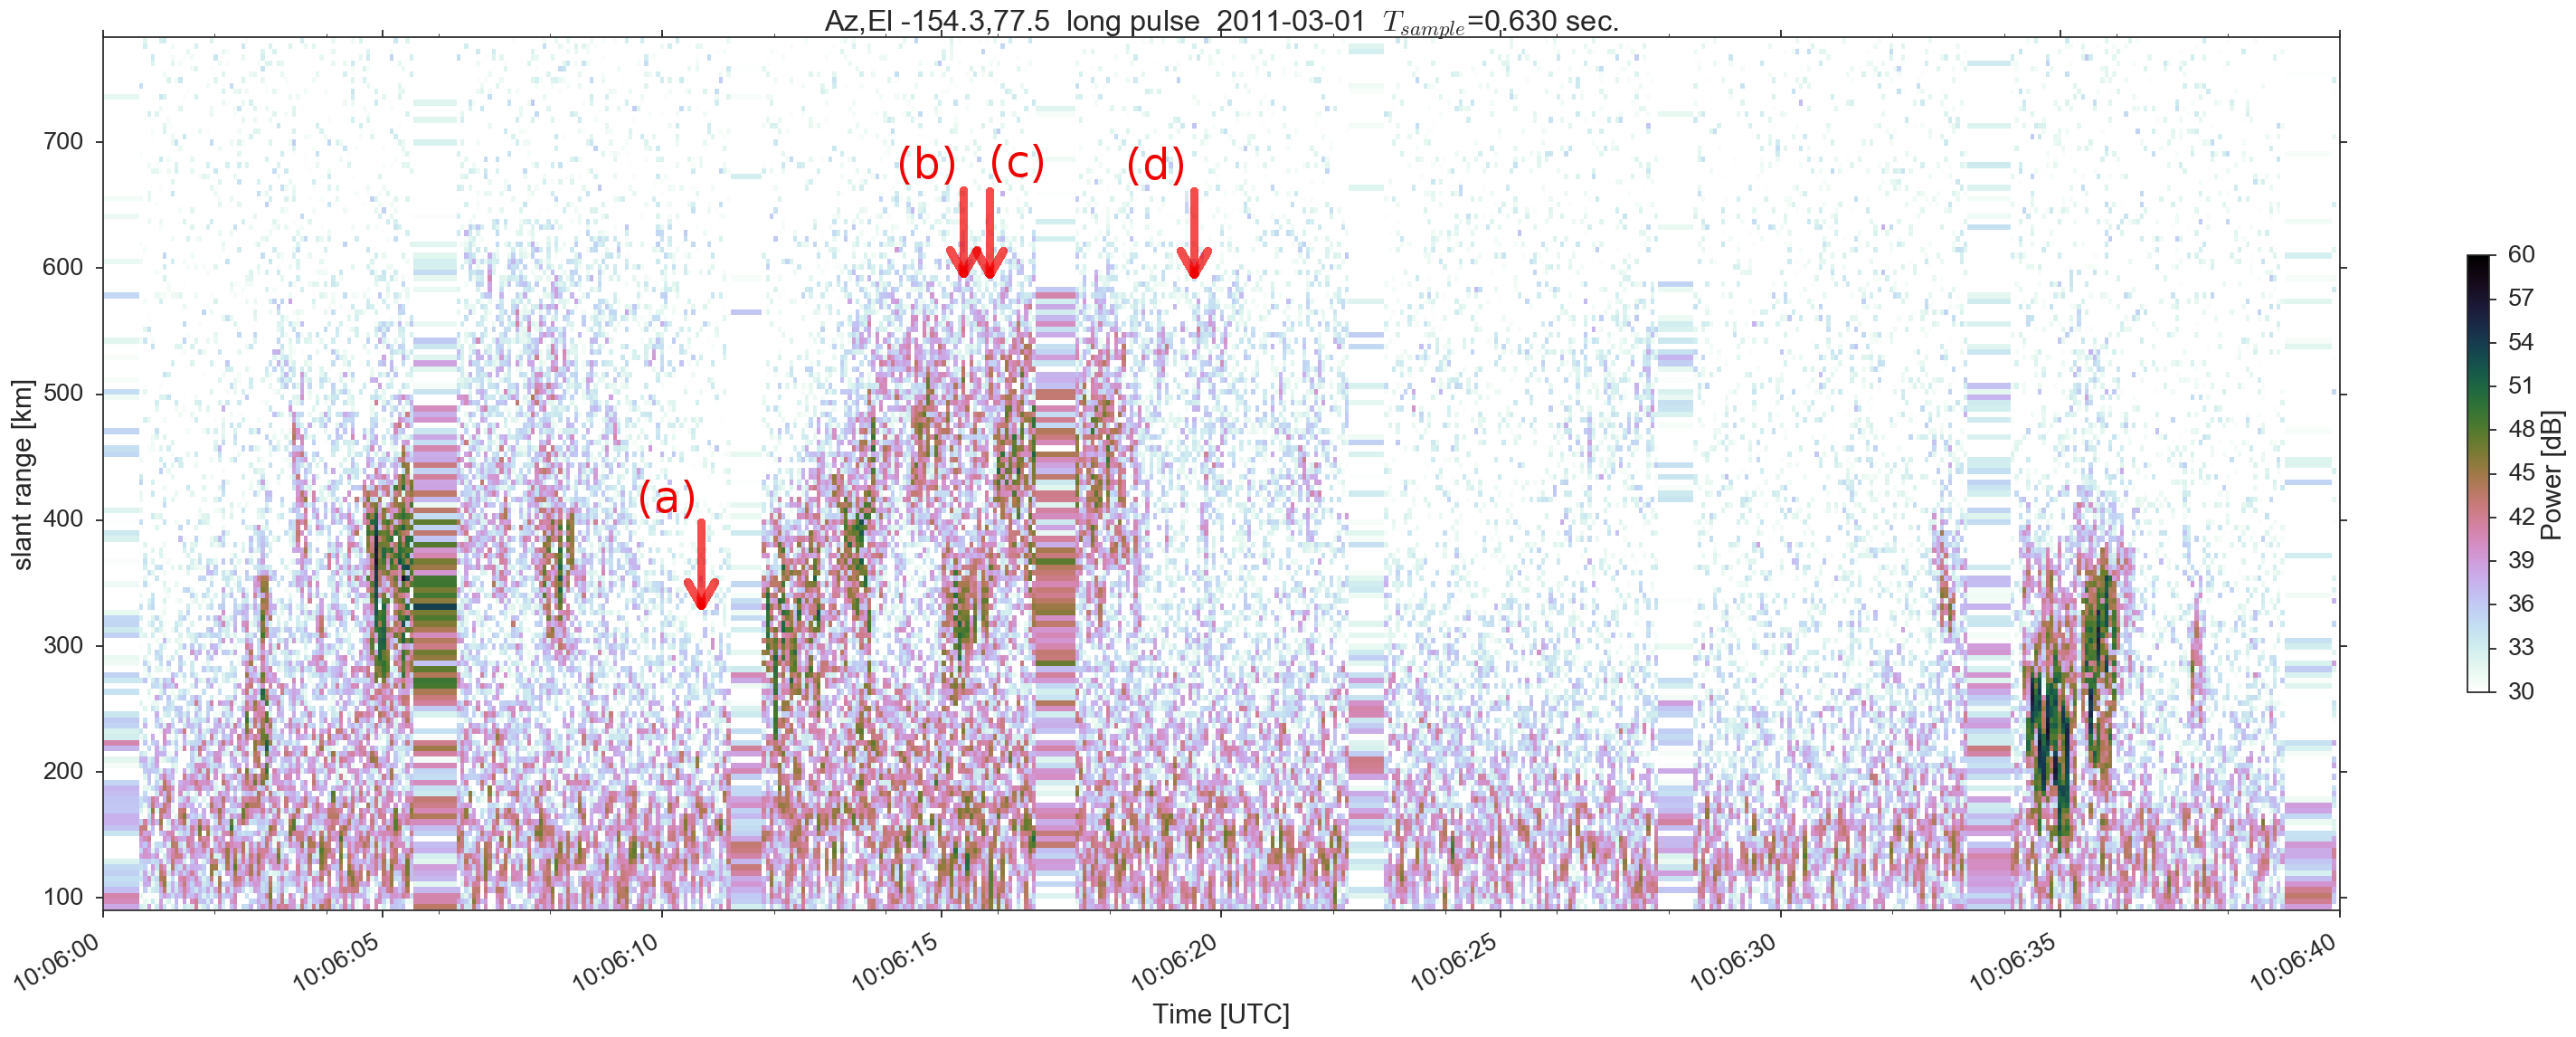
\includegraphics[width=\columnwidth,trim=0 50 0 0]{gfx/2011-03-01/power_longpulse2011-03-0110-06-00}\\
    {\large(e)}
    \vspace{0.1cm}
    
    \caption{Flaming auroral arc sequence at PFISR on March 1, 2011, 10:06 UTC. 
        (a) shows pre-Alfvénic arc configuration. 
        (b) F-region irregularities are observed in the ISR power (e) with the arrival of high-energy DAW accelerated electron. 
        (c) \unit[400]{ms} later, the low-energy Alfvénic flux dominates as the apparent peak altitude of prompt emissions rises rapidly. 
        (d) the Alfvénic particle packet has vanished. 
        (e) ISR backscatter showing three NEIAL events in series--video only available for middle event.}
    \label{fig:20110301a}
\end{sidewaysfigure}

\begin{figure}\centering
    % Psd
    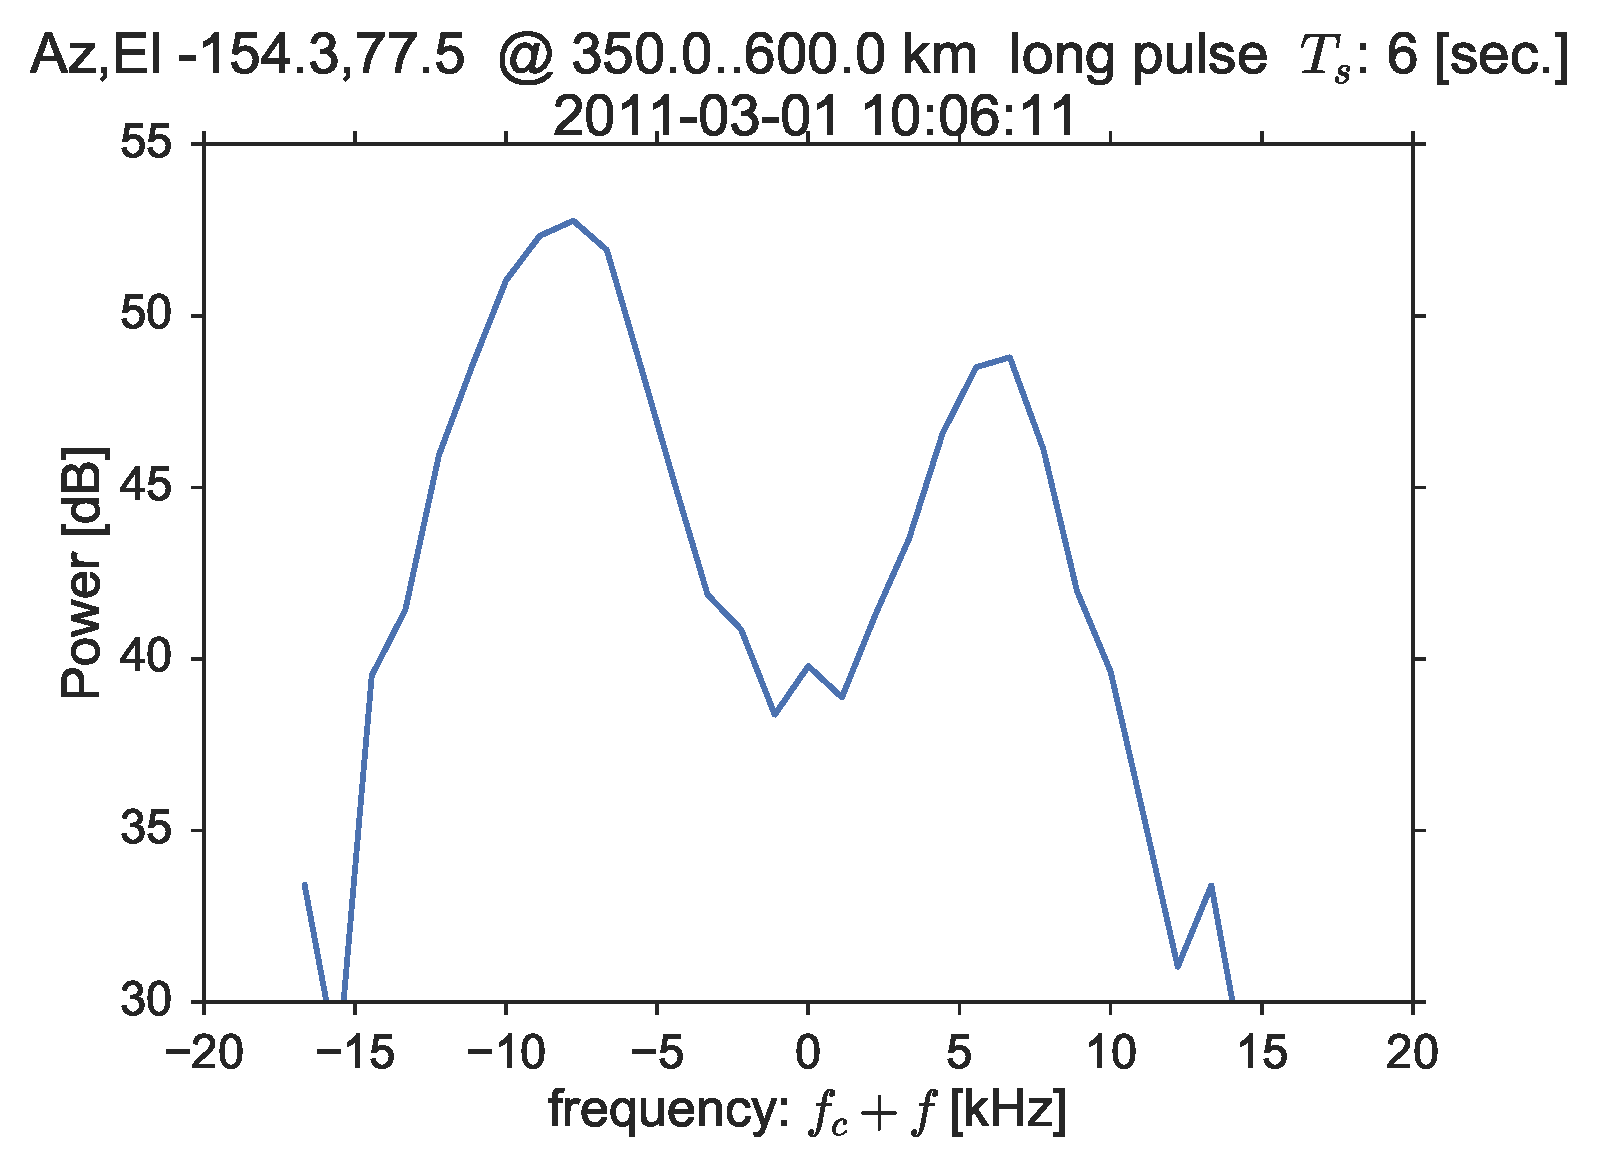
\includegraphics[width=0.5\columnwidth,trim=0 50 0 0]{gfx/2011-03-01/acfslice_longpulse2011-03-0110-06-11}
    
    \vspace{-1cm}(a)
    \vspace{1cm}
    
    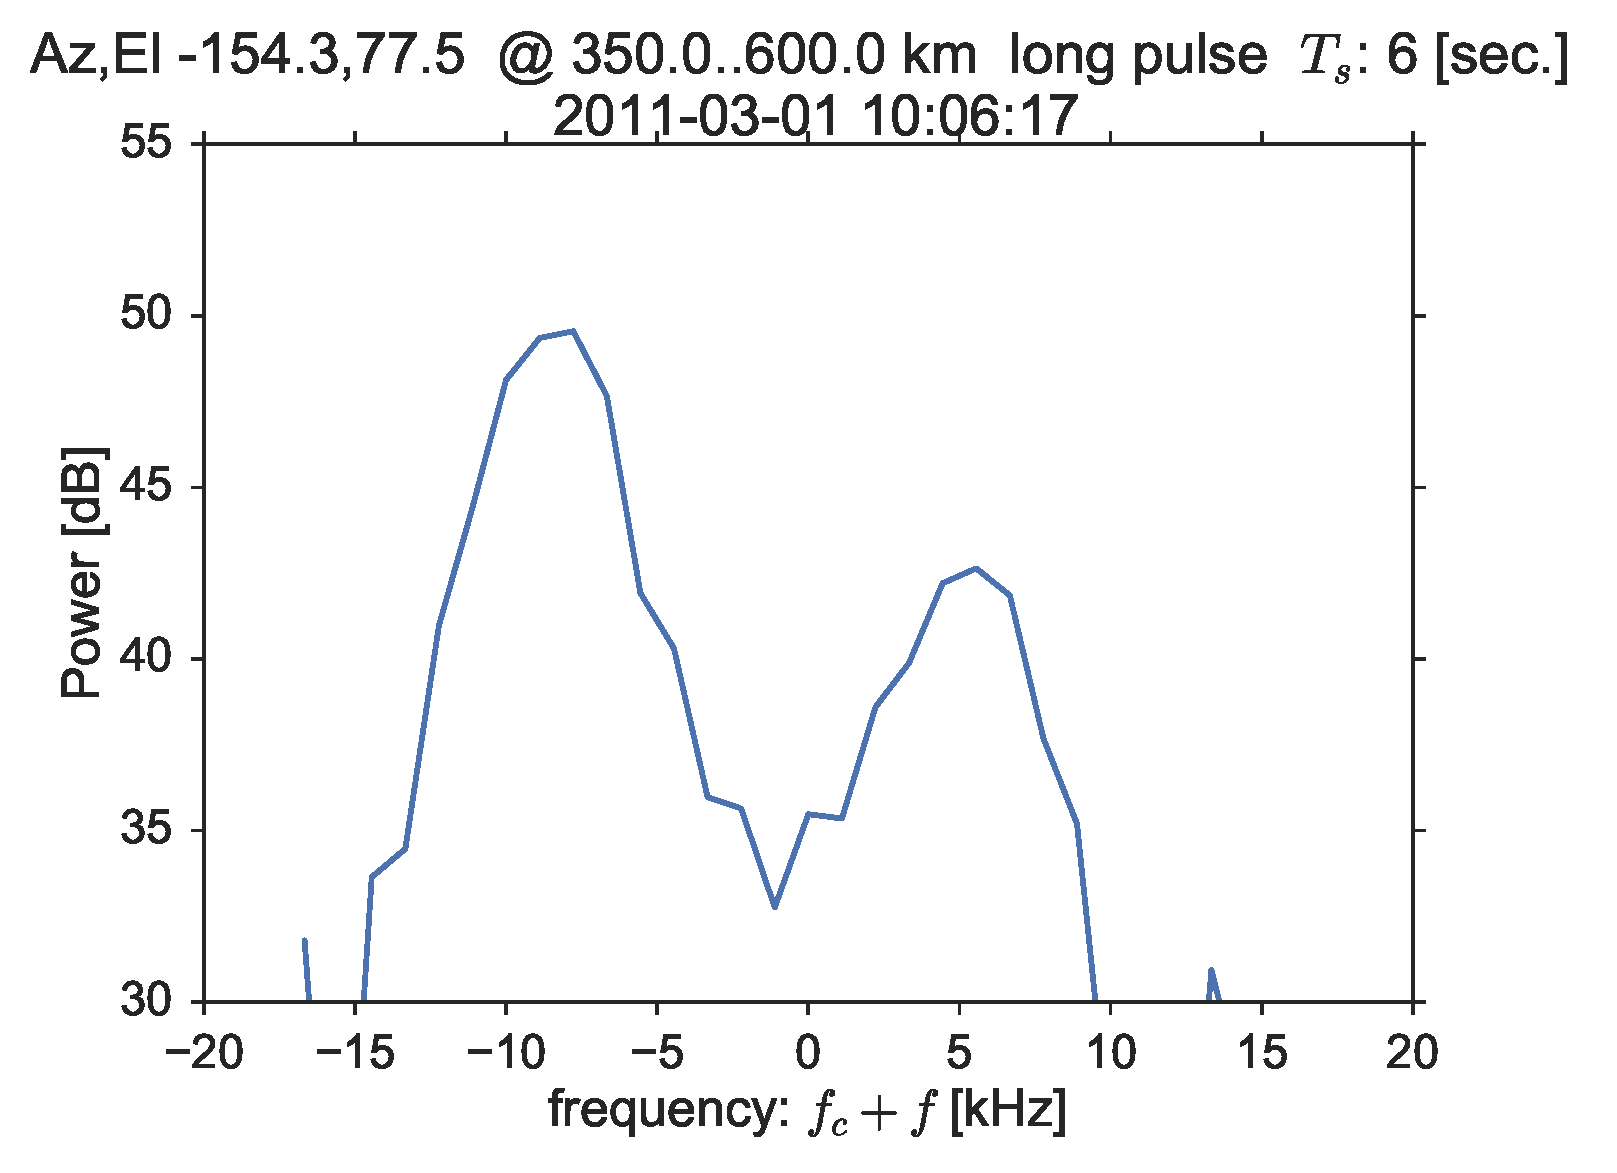
\includegraphics[width=0.5\columnwidth,trim=0 50 0 0]{gfx/2011-03-01/acfslice_longpulse2011-03-0110-06-17}
    
    \vspace{-1cm}(b)
    \vspace{1cm}
    
    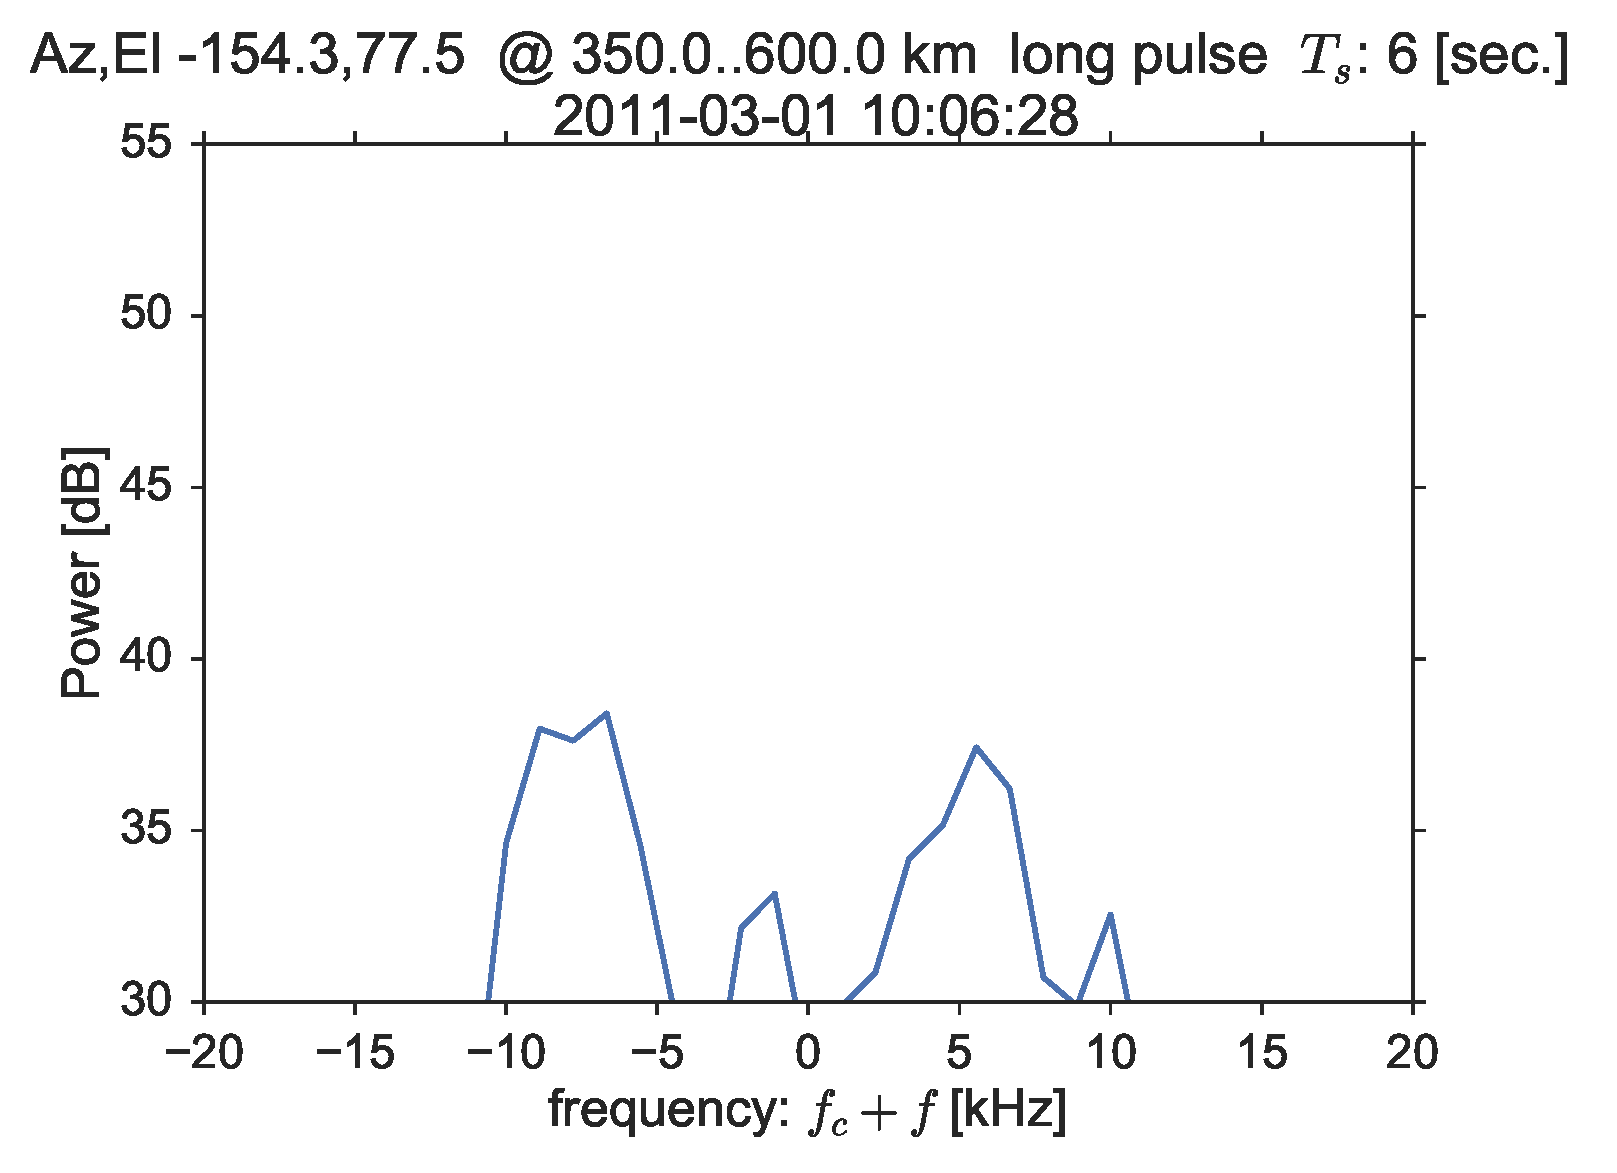
\includegraphics[width=0.5\columnwidth,trim=0 50 0 0]{gfx/2011-03-01/acfslice_longpulse2011-03-0110-06-28}
    
    \vspace{-1cm}(c)
    \vspace{1cm}
    
	%(a)\hspace{0.275\columnwidth}(b)\hspace{0.275\columnwidth}(c)
	
	\caption{Flaming auroral arc sequence at PFISR on March 1, 2011. 
    (a,b) show enhanced negative frequency shift ion-acoustic line. 
    (c) shows normal ion-acoustic line.}
    \label{fig:20110301b}
\end{figure}

Only a single high-speed sCMOS was running at 30 frames/s, in burst recording mode of several seconds each manual record start.
Context for the event is provided by PF-DMSP in Figure~\ref{fig:msp20110301} and GIMA in Figure~\ref{fig:mag20110301}.
\begin{figure}\centering
    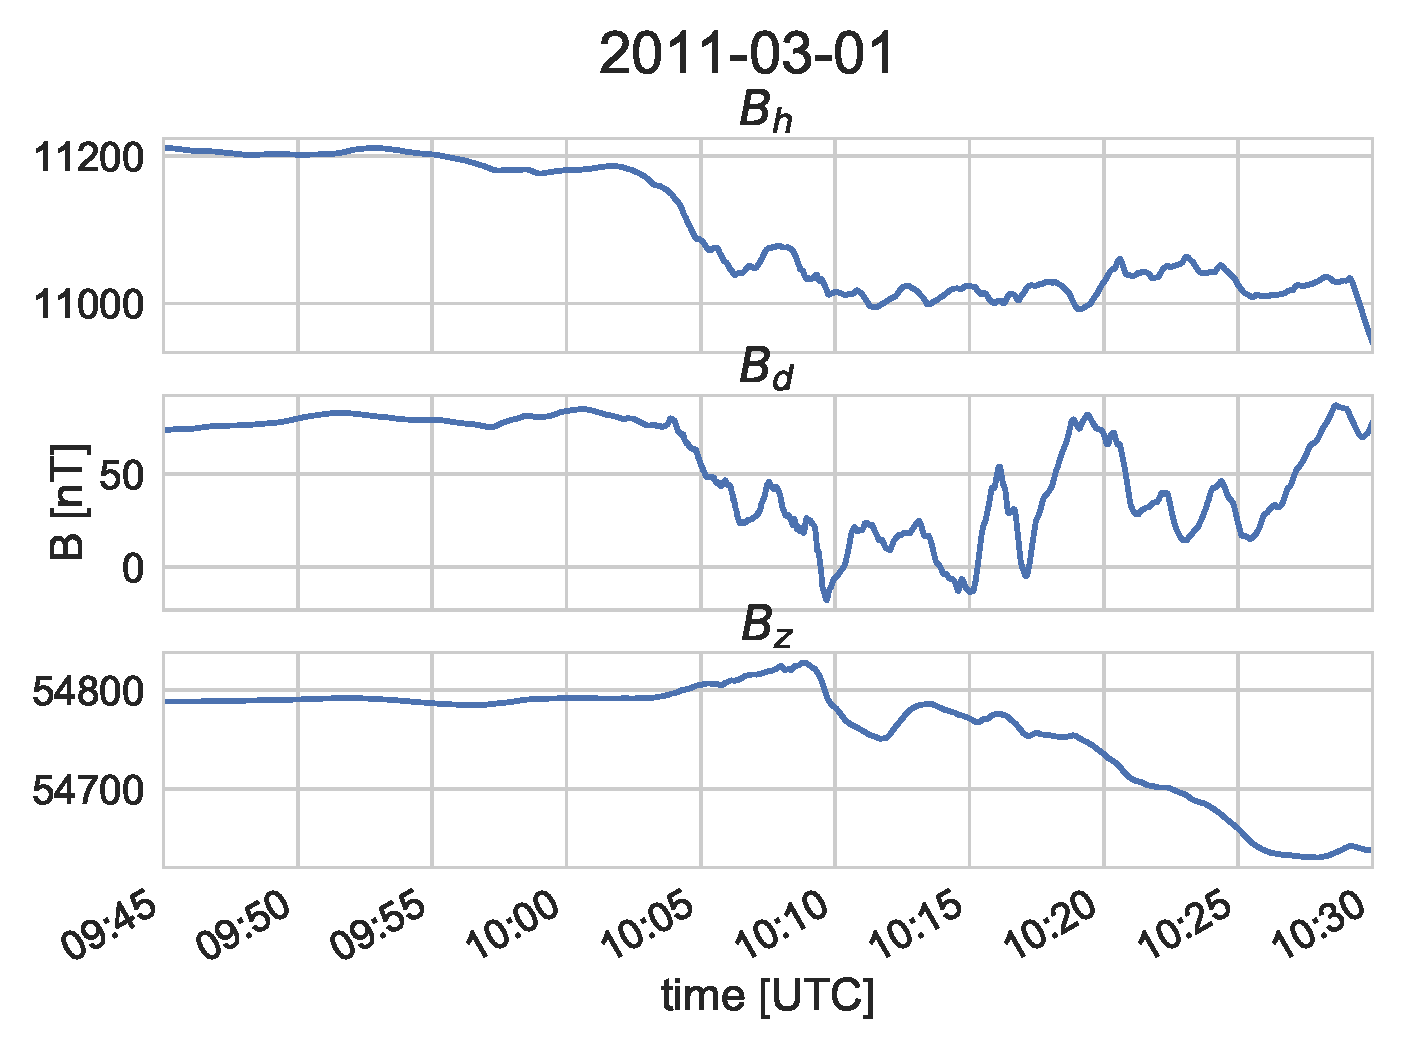
\includegraphics[width=\columnwidth]{gfx/2011-03-01/mag}
    \caption{Quiet conditions before the flaming auroral event are perturbed during the 2011-03-01 substorm.}
    \label{mag:20110301}
\end{figure}
The PF-DMSP spectrum of Figure~\ref{fig:msp20110301} had $I_{555.7}$ and $I_{427.8}$ available.
\begin{figure}\centering
    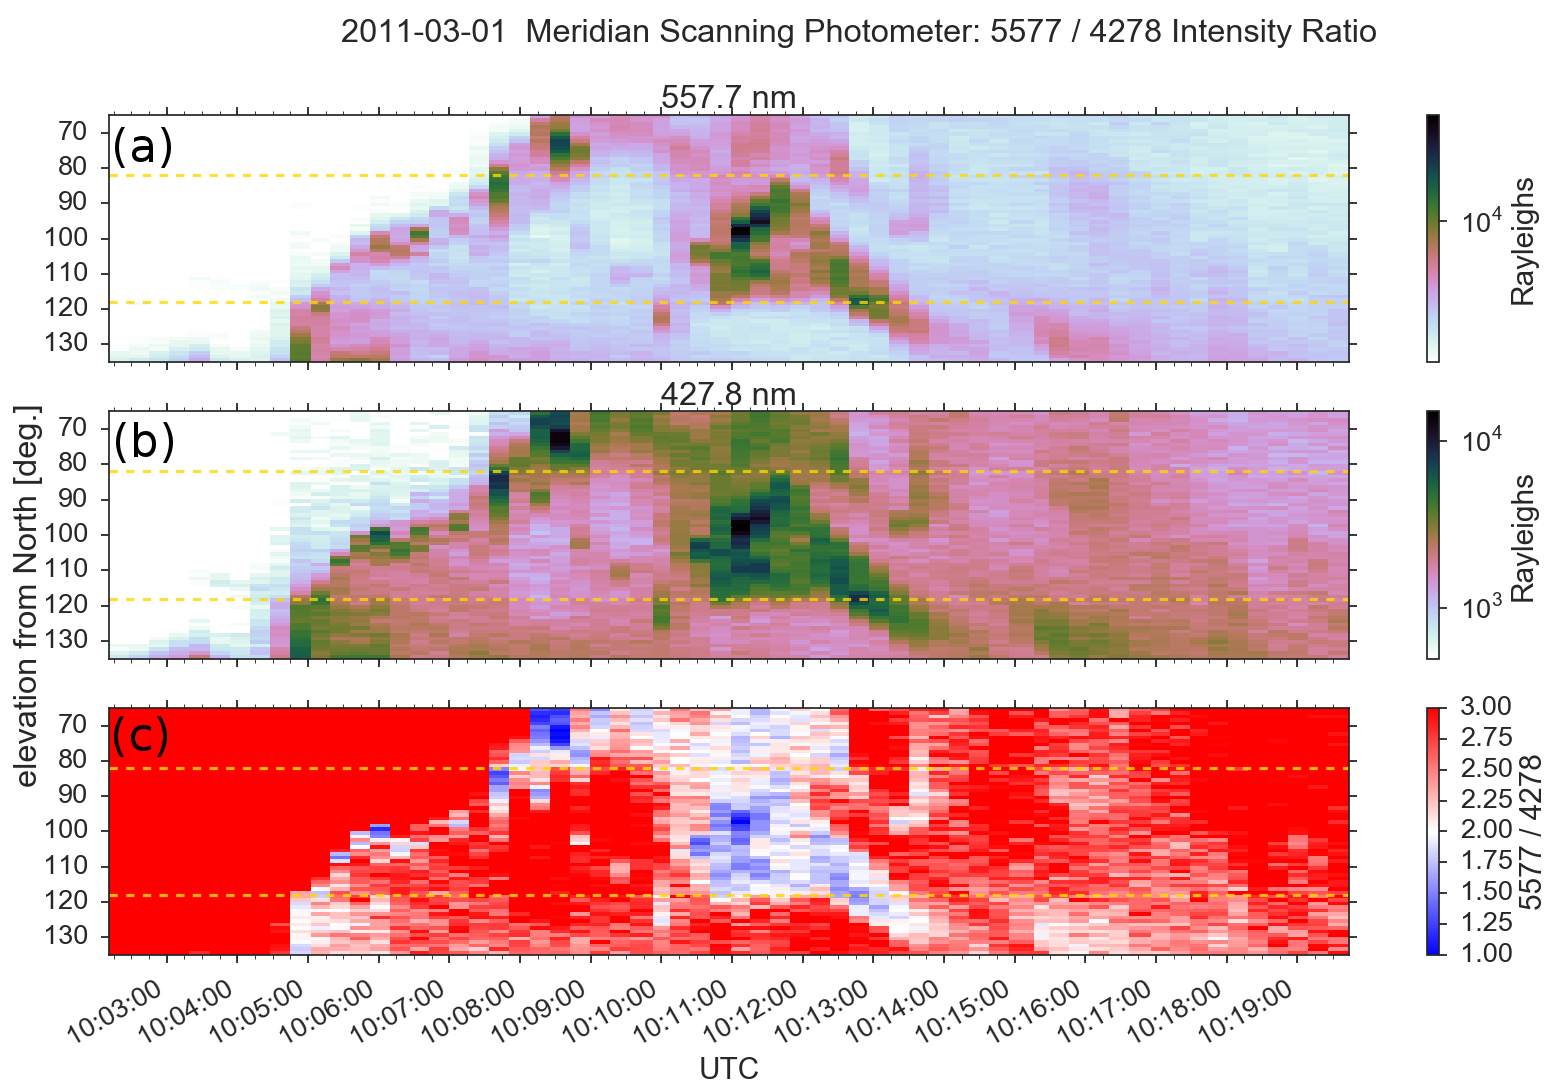
\includegraphics[width=\columnwidth]{gfx/2011-03-01/msp_ratio}
    \caption{PF-DMSP (a) $I_{555.7}$ and (b) $I_{427.8}$ with ratio (c) $I_{555.7} / I_{427.8}$. Around 10:06 and 10:11 UTC  intensifications near magnetic zenith indicates large increase in characteristic energy.}
    \label{fig:msp20110301}
\end{figure}
According to \citet{rees1974}, the magnetic zenith energies are on the order of \unit[5..10]{keV} during this event.
The PF-DMSP data is highly smeared in time across this event.
\citet{dahlgren2013} provided estimates using assumptions on the starting altitude of the flaming feature in a single-camera data inversion.
HiST was designed to study this type of event, with long-term automated recording so that events are not missed and the precipitation energy dynamics can be examined in more quantitative detail.